\documentclass{article}

% Document information
\title{Multi-view Clustering For COPDGene 10,000 Dataset}
\author{Yale Chang}
\date{}

% Packages
%\usepackage[margin=1.0in]{geometry}
\usepackage{amsmath}
\usepackage{amssymb}
\usepackage{graphicx}
\usepackage{caption}
\usepackage{subcaption}

% Define new command
\newcommand{\HSIC}{\mathrm{HSIC}}
\newcommand{\NHSIC}{\mathrm{NHSIC}}
\newcommand{\Tr}{\mathrm{Tr}}

\begin{document}

% Title
\maketitle

\section{Dataset Descritption}
\textbf{Dataset File:} dataset\_complete\_knn\_windsor\_11-18-13.csv\\
\textbf{Feature Annotation File:} features\_included\_info\_mhc20131104.txt\\
\textbf{Details:} There are altogether 8760 samples and 211 features in the dataset file. According to the annotation information provided in the feature annotation file, 63 continuous features(without `Times' variables) are selected for subsequent analysis. Samples in dataset file can be divided into training set and test set according to the value of variable `RandomGroupCode'. There are 4413 training samples. In the end, we use a dataset consisting of 4413 training samples and 63 annotated features .

\section{Features Similarity matrix}
\subsection{HSIC}
HSIC(Hilbert-Schmidt Independence Criterion) can be used to compute non-linear dependencies between features.Note that correlation coefficient can only capture linear dependencies between random variables and mutual information requires estimating the joint distribution of the random variables. While HSIC can measure dependence between random variables without explicitly estimating joint distributions. We can empirically estimate the HSIC by:\\
\begin{equation}
	\label{eq_hsic}
	\HSIC(Z,F,G)=(n-1)^{-2}\Tr(K_1HK_2H)
\end{equation}
where $Z = \{(x_1,y_1),\cdots,(x_n,y_n)\}$ represents $n$ observations of random variable $X$ and $Y$, $F$ and $G$ are kernel spaces on $X$ and $Y$ respectively. $K_1,K_2\in \mathrm{R}^{n\times n}$ are Gram matrices, $(K_1)_{ij}=k_1(x_i,x_j),(K_2)_{i,j}=k_2(y_i,y_j),(H)_{ij}=\delta_{ij}-n^{-1}$.\\ 
\\
Since we're working with continuous features, Gaussian kernel can be used in computing Gram matrices:\\
\begin{equation}
	K(x_i,x_j) = \exp(-\frac{\|x_i-x_j\|^2}{2\sigma_{HSIC}^2})
\end{equation} 
\\
In the experiment, since the number of features is 63, we can get a $63\times 63$ similarity matrix $S_f$, where $S_{f}(i,j)$ represents the dependency between $i$-th feature and $j$-th feature.\\
\\
However, by observing equation (\ref{eq_hsic}), the diagonal elements of matrix $S_f$ are not the same. To make the similarity between two features that are exactly the same to be 1, we can introduce normalized HISC:
\begin{equation}
	\NHSIC(X,Y) = \frac{\HSIC(X,Y)}{\sqrt{\HSIC(X,X)\cdot \HSIC(Y,Y)}}
\end{equation}  

\subsection{Number of Feature Clusters}
Spectral clustering can be applied to cluster features. It's a common practice to determine the number of clusters by observing the eigenvalues of Laplacian matrix in spectral clustering.

\begin{figure}
\centering
	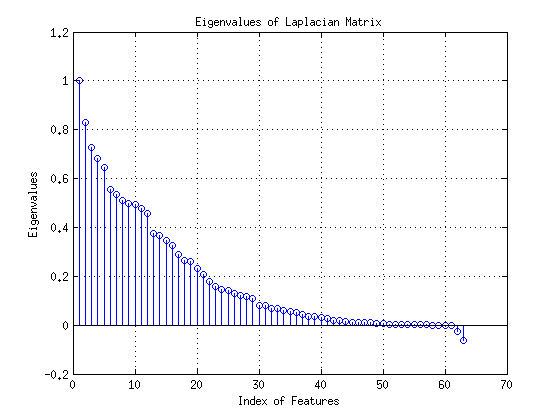
\includegraphics[width=1.\linewidth]{plt_eigenvalues.png}
	\caption{Eigenvalues of Laplacian Matrix}
	\label{fig_1}
\end{figure}

\begin{figure}
\centering
	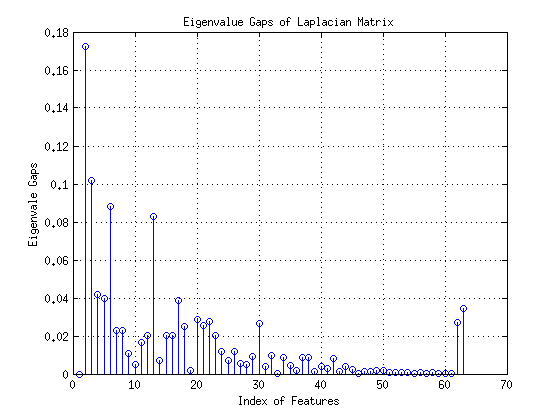
\includegraphics[width=1.\linewidth]{plt_eigenvalue_gaps.png}
	\caption{Eigenvalue Gaps of Laplacian Matrix}
	\label{fig_2}
\end{figure}

From Figure(\ref{fig_1}) and Figure(\ref{fig_2}) We can observe that the top eigenvalue gaps appears at 1-2(0.1723), 2-3(0.1021), 5-6(0.0880), 12-13(0.0828). Therefore, we will set the number of feature clusters to be \textbf{2,5,12} respectively and output the plot of corresponding similarity matrix.
\begin{figure}
\centering
	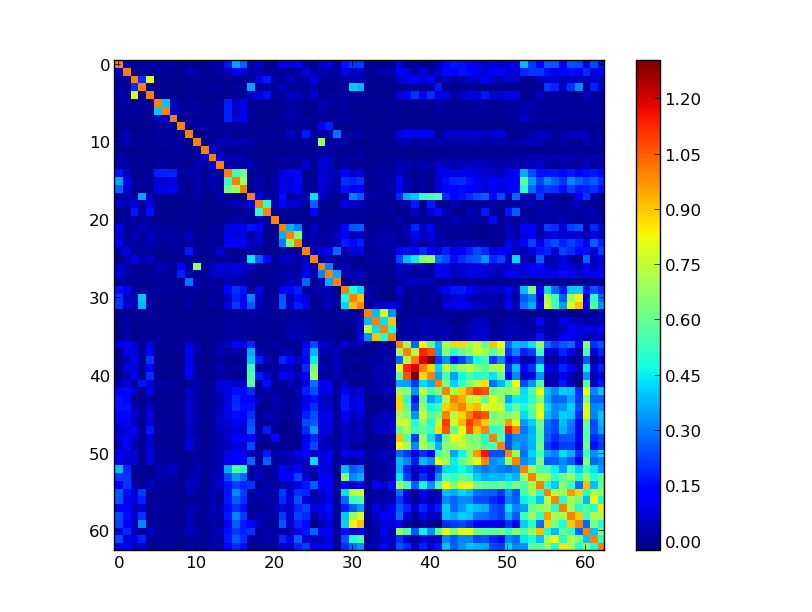
\includegraphics[width=1.\linewidth]{plt_n_clusters_f_2.png}
	\caption{Similarity Matrix when Number of Feature Clusters = 2}
	\label{fig_3}
\end{figure}

\begin{figure}
\centering
	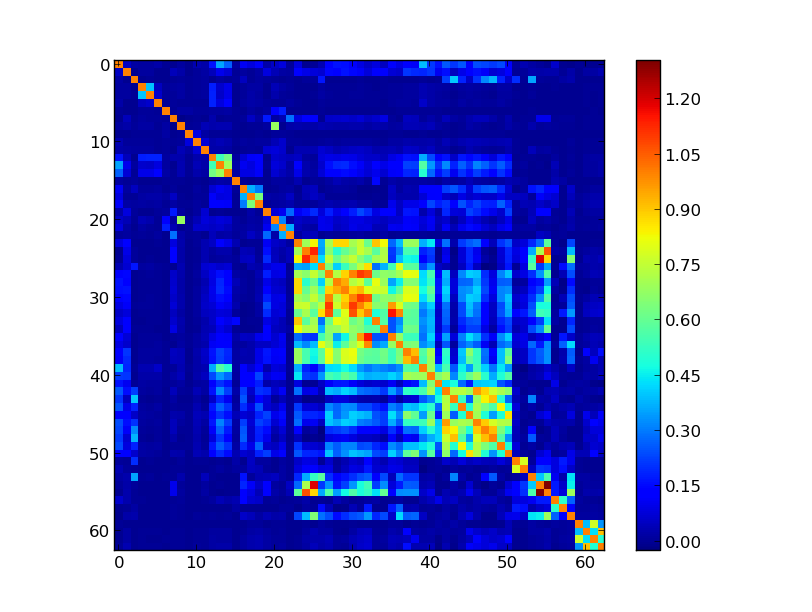
\includegraphics[width=1.\linewidth]{plt_n_clusters_f_5.png}
	\caption{Similarity Matrix when Number of Feature Clusters = 5}
	\label{fig_4}
\end{figure}

\begin{figure}
\centering
	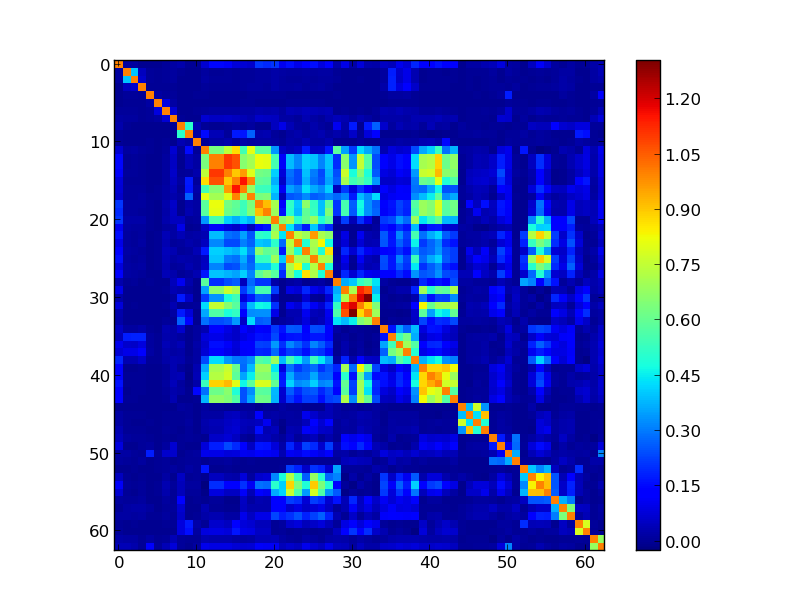
\includegraphics[width=1.\linewidth]{plt_n_clusters_f_12.png}
	\caption{Similarity Matrix when Number of Feature Clusters = 12}
	\label{fig_5}
\end{figure}
By comparing Figure(\ref{fig_3}),Figure(\ref{fig_4}) and Figure(\ref{fig_5}), we can conclude it's more resonable to set the number of feature clusters to be 5.

\subsection{Analyze Feature Clusters}
When we set the number of feature clusters to be 5, the details of feature clusters are as following:\\

\begin{table}[ht]\scriptsize
\caption{Feature Clusters}
\begin{tabular}{c c c c c}
\hline\hline
Cluster 1 & Cluster 2 & Cluster 3 & Cluster 4 & Cluster 5\\[1ex]
\hline
distwalked & pctEmph\_Slicer & BODE & Weight\_KG & deltaFEV1\\
Resting\_SaO2 & Insp\_Below910\_Slicer & FEV1pp\_utah& BMI& deltaFVC\\
Height\_CM & Slicer\_15pctIn\_Total & FVCpp\_utah& TLC\_Slicer& BDR\_pct\_FEV1\\
CoughNumYr & FRC\_Slicer & FEV1\_utah & Insp\_Below856\_Slicer& BDR\_pct\_FVC\\
PhlegmNumYr & pctGasTrap\_Slicer & FVC\_utah & Slicer\_IntensityStdDev\_In & \\
NumEpisodeLastYr & Exp\_Below950\_Slicer & PEF\_utah & Slicer\_IntensityStdDev\_Ex & \\
SmokStartAge & Exp\_Below910\_Slicer & PEF2575\_utah & TLCpp\_race\_adjusted & \\
CigPerDaySmokNow & Exp\_Below856\_Slicer & pre\_FEV1 & & \\
CigPerDaySmokAvg & Slicer\_15pctEx\_Total & pre\_FEV6 & & \\
OthSmokChildYrs & Slicer\_IntensityMean\_Ex & pre\_FVC && \\
OthSmokYrs & pctEmph\_UpperThird\_Slicer & pre\_PEF& & \\
ExpSmokAtWorkYr & pctEmph\_LowerThird\_Slicer & pre\_PEF2575 & & \\
SGRQ\_scoreSymptom & Slicer\_ExpInspMeanAtten\_ratio & & & \\
SGRQ\_scoreActive & FRCpp\_race\_adjusted & & & \\
SGRQ\_scoreImpact & FEV1\_FVC\_utah & & & \\
UpperThird\_LowerThird\_Slicer & pre\_FEV1\_FVC & & & \\
Pi10\_SRWA & & & & \\
Pi15\_SRWA & & & & \\
WallAreaPct\_seg & & & & \\
Age\_Enroll & & & & \\
ATS\_PackYears & & & & \\
Duration\_Smoking & & & & \\
YearsSinceQuit & & & & \\
\hline
\end{tabular}
\label{table:dist_cluster_labels_gold_1}
\end{table}

\subsection{Clustering on Samples with Different Feature Sets}
We compare the clustering results on samples with Feature Set 2, Feature Set 3 and the whole Feature Set. At the same time, we vary the number of clusters. We also visualize the clustering results under different conditions in 2D and 3D projection spaces by applying kernel PCA. We also cluster with features selected by backward search and forward search with different supervisions.The results are presented in a set of figures. 
\end{document}